%%% Décommenter pour une présentation
\documentclass{beamer}
%%%

%%% Décommenter pour avoir un article
%\documentclass[handout]{beamer}
%\usepackage{pgfpages}
%\pgfpagesuselayout{2 on 1}[a4paper,border shrink=5mm]
%\setbeameroption{show notes on second screen=bottom} % Beamer manual, section 19.3
%%%

%%%%%%%%%%%%%%%%%%%%%%%%%%%%%%%%%%%%%%%%%%%%%%%%%%%%%%%%%%%%%%%%%%%%%%
% NE PAS MODIFIER CETTE PARTIE

\usetheme{Antibes}
\usepackage[utf8]{inputenc}
\usepackage[french]{babel}
\usepackage[T1]{fontenc}
\usepackage{amsmath}
\usepackage{amsfonts}
\usepackage{amssymb}
\usepackage{graphicx}
\usepackage{listings}
\usepackage{hyperref}
\usepackage[backend=bibtex]{biblatex}

%%%%%%%%%%%%%%%%%%%%%%%%%%%%%%%%%%%%%%%%%%%%%%%%%%%%%%%%%%%%%%%%%%%%%%
% SI BESOIN
%\addbibresource{biblio.bib}
%\nocite{*}

\graphicspath{{graphics/}}

\hypersetup{pdfstartview={Fit}}



\AtBeginSection[]{
  \begin{frame}
  \vfill
  \centering
  \begin{beamercolorbox}[sep=8pt,center,shadow=true,rounded=true]{title}
    \usebeamerfont{title}\insertsectionhead\par%
  \end{beamercolorbox}
  \vfill
  \end{frame}
}

\setbeamertemplate{note page}[plain] % Beamer manual, section 19.1
\newlength{\parskipbackup}
\setlength{\parskipbackup}{\parskip}
\newlength{\parindentbackup}
\setlength{\parindentbackup}{\parindent}
\newcommand{\baselinestretchbackup}{\baselinestretch}
\usetemplatenote{\rmfamily \scriptsize%
  \setlength{\parindent}{1em} \setlength{\parskip}{1ex}%
  \renewcommand{\baselinestretch}{1}%
  \noindent \insertnote%

  \setlength{\parskip}{\parskipbackup}%
  \setlength{\parindent}{\parindentbackup}%
  \renewcommand{\baselinestretch}{\baselinestretchbackup}%
}

\logo{
	
\includegraphics[scale=0.05]{eurecom.jpg}
} 
\institute[EURECOM]{\textbf{EURECOM}}



%%%%%%%%%%%%%%%%%%%%%%%%%%%%%%%%%%%%%%%%%%%%%%%%%%%%%%%%%%%%%%%%%%%%


\date{January 18\textsuperscript{th}, 2018}

\author{Laila SALHI\\Clément TRASSOUDAINE}
\title{
	\textbf{Machine-Learning for Neuroimaging}\\
	-\\ 
	\textit{State of the art}
}




\begin{document}

\frame{\titlepage}
\frame{\tableofcontents}



%%%%%%%%%%%%%%%%%%%%%%%%%
%%%%% INTRODUCTION %%%%%%
%%%%%%%%%%%%%%%%%%%%%%%%%
\section{Introduction}

\begin{frame}
\frametitle{Neuroimaging 101}
\begin{minipage}{0.45\linewidth}
{\textbf{NMR Techniques}}
\begin{itemize}
\item MRI
	\begin{itemize}
	\item GMD
	\end{itemize}
\item fMRI
	\begin{itemize}
	\item BOLD
	\end{itemize}
\end{itemize}
\end{minipage}
\hfill
\begin{minipage}{0.45\linewidth}
{\textbf{Other techniques}}
\begin{itemize}
\item PET
\item MEG/EEG
\item NIRS/SPIR
\item ...
\end{itemize}
\vfill
\end{minipage}
\vfill
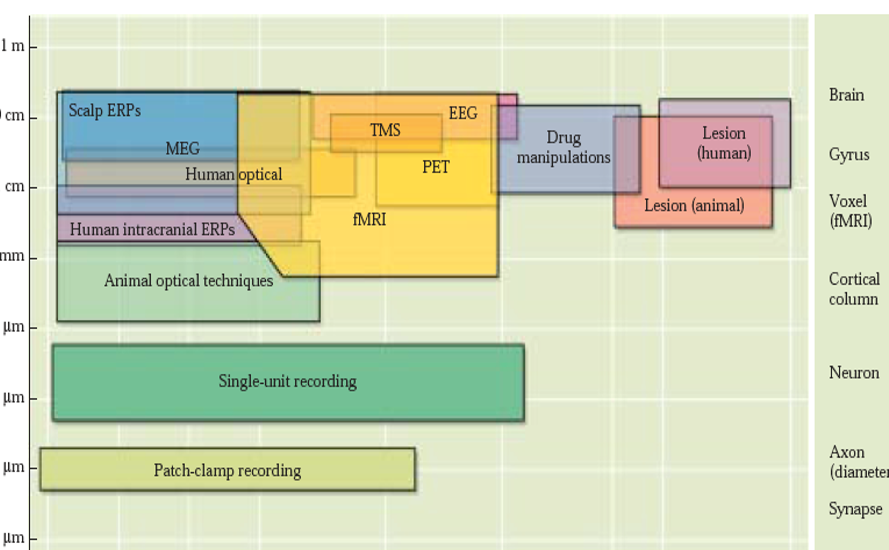
\includegraphics[scale=.3]{resolutions.png}

\end{frame}



\note{

Gray matter : neurons
MRI : Magnetic resonnance imaging
PET : Positron emetion tomography
MEG : magnetoencephalography
NIRS/SPIR optical techniques
Talk about voxels
}

%%%%%%%%%%%%%%%%%%%%%%%%%
%%%%%     BODY     %%%%%%
%%%%%%%%%%%%%%%%%%%%%%%%%

\section{Techniques}

\subsection{A statistical view}

%Selecting part of interest (searchlight, K-best)
\begin{frame}
\frametitle{Selecting part of interest}
\begin{minipage}{.45\linewidth}
\centering
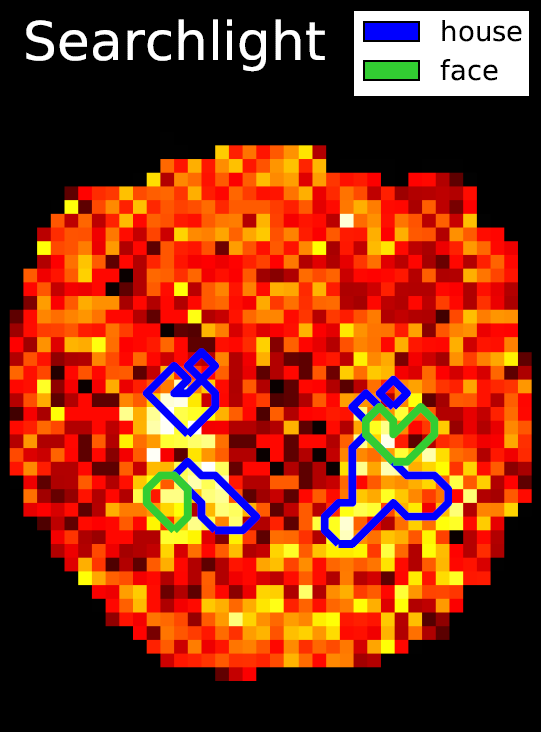
\includegraphics[scale=0.3]{searchlight.png}
\end{minipage}
\hfill
\begin{minipage}{.45\linewidth}
\centering
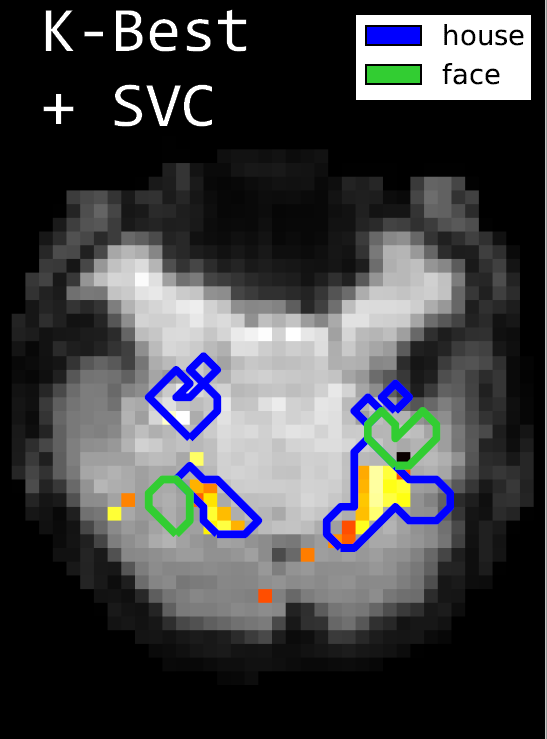
\includegraphics[scale=0.3]{kbest.png}
\end{minipage}
\footnotetext[1]{
\tiny
Abraham, Alexandre et al. “Machine Learning for Neuroimaging with Scikit-Learn.” Frontiers in Neuroinformatics 8 (2014): 14. PMC. Web. 28 Oct. 2017.
}
\end{frame}

\note{
Huge amount of voxels --> computationally costly
Need to find a subset that is representative for the data. (it also removes the noise)
Here are two techniques (the most used in Neuroimaging), namely Searchlight and K-best to find the voxels of interest.
These are z-slice subsets of a brain mri.

Let's start with K-best. The idea is to compute the variance over the whole dataset for each voxel and to select only K best variance. These are most likely to be differences that interest us. However this requires to have a well balanced dataset to be sensitive only to the phenomenon that we want to observe. 
Then the colors that you are the weights found by the classifier to pixels this is what we will see a little bit later.

The major difference between KBest and searchlight is that there is a consideration of voxel's neighbours in searchlight. When computing the variance, it takes into account the neigbours and is then way less sensitive to noise. This is also way more computationally expensive. Searchlight then gives a score of interest to all of the voxels and we can use it as is for finding regions of interest or threshold it and use a classifier on the remaining voxels.
}

\subsection{Regression and Classification}
\begin{frame}
\frametitle{Regression and Classification}
\begin{itemize}
\item Support Vector Machine 
	\begin{itemize}
	\item Find an hyperplane that maximizes the distance of the closest points.
    \item Focus on the max margin size.
	\end{itemize}
\item Logistic Regression
	\begin{itemize}
	\item Find an hyperplane that maximize the probability ( $P(Y=y|X)$ ) for points to be on the good side.
    \item Uses a likelihood function.
	\end{itemize}
\end{itemize}

\begin{center}
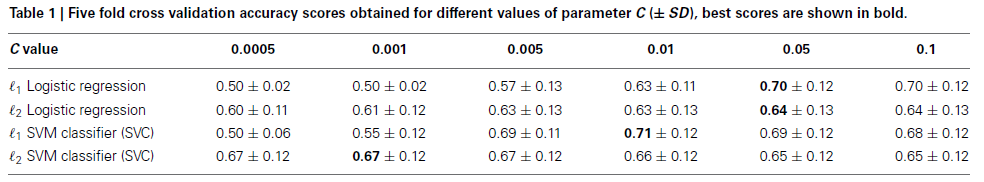
\includegraphics[scale=.48]{LRvsSVM.png}
\end{center}

\end{frame}

\begin{frame}
\frametitle{Semi-supervised learning}
\begin{minipage}{.55\linewidth}
\begin{itemize}
\item Inputs: Labeled and non-labeled data
\item Clustering for classification\\
LDS : Low-density separation\\
TSVM : Transductive SVM
\end{itemize}
\end{minipage}
\hfill
\begin{minipage}{.4\linewidth}
\centering
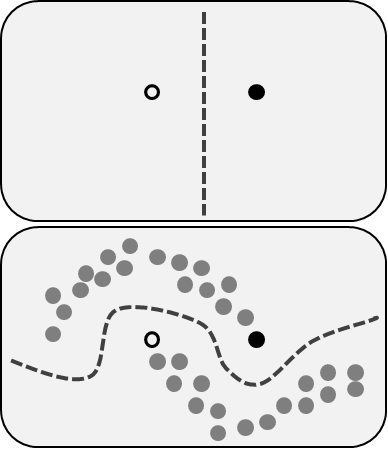
\includegraphics[scale=.37]{semisupervised.png}
\end{minipage}

\footnotetext[1]{
\tiny
By Techerin - Own work, CC BY-SA 3.0, https://commons.wikimedia.org/w/index.php?curid=19514958
}
\end{frame}

\subsection{Clustering}

\begin{frame}
\frametitle{Extracting brain's network with ICA}
\begin{minipage}{.50\linewidth}
\begin{itemize}
\item Limits Neuroimaging
\item Need for cognitive ontology (BrainMap Database)
\item Improving Reverse Inference
\end{itemize}
\end{minipage}
\hfill
\begin{minipage}{.45\linewidth}
\centering
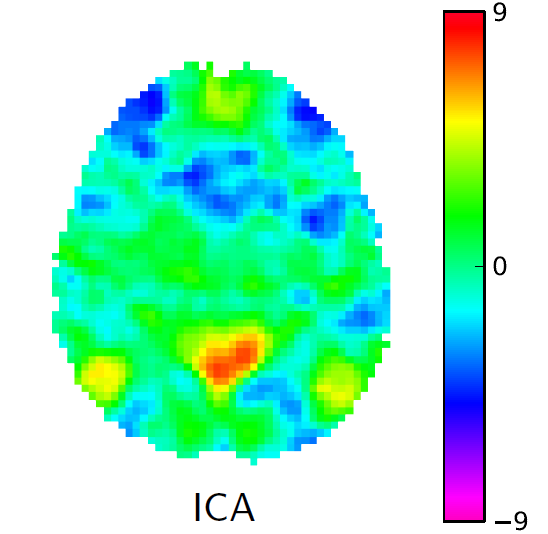
\includegraphics[scale=0.4]{ICA.png}
\end{minipage}
\footnotetext[1]{
\tiny
Abraham, Alexandre et al. “Machine Learning for Neuroimaging with Scikit-Learn.” Frontiers in Neuroinformatics 8 (2014): 14. PMC. Web. 28 Oct. 2017.
}

\end{frame}
% ICA

\begin{frame}
\frametitle{Clustering with K-means approach}
\begin{itemize}
\item Each voxels is assigned to the nearest center, forming clusters
\end{itemize}
\centering
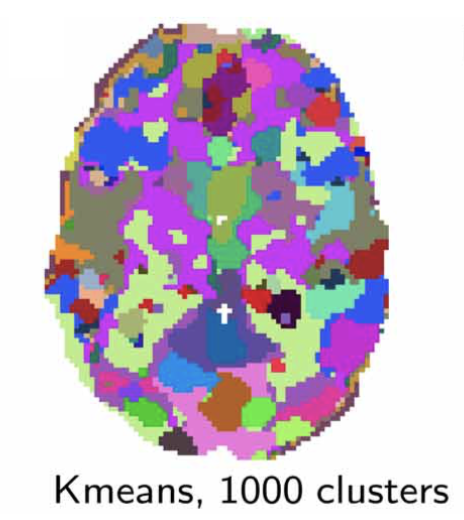
\includegraphics[scale=0.5]{K-means1.png}
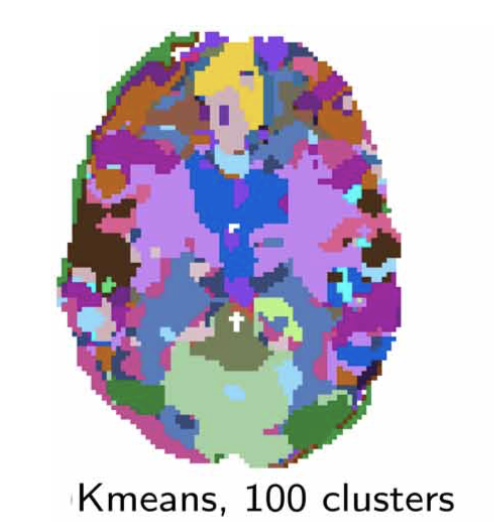
\includegraphics[scale=0.5]{K-means2.png}
\footnotetext[1]{
\tiny
Abraham, Alexandre et al. “Machine Learning for Neuroimaging with Scikit-Learn.” Frontiers in Neuroinformatics 8 (2014): 14. PMC. Web. 28 Oct. 2017.
}
\end{frame}
% K-Means

%%%%%%%%%%%%%%%%%%%%%%%%%
%%%% TECHNICALITIES %%%%%
%%%%%%%%%%%%%%%%%%%%%%%%%

\section{Case studies}

\subsection{Diseases and condition prediction}

\begin{frame}
\frametitle{Age and dementia prediction}
\begin{minipage}{.45\linewidth}
\begin{itemize}
\item Record MRI based on GMD.
\item Train a dementia classification model and an age regression model.
\item Look at the involved parts of the brain.
\end{itemize}
\end{minipage}
\hfill
\begin{minipage}{.45\linewidth}
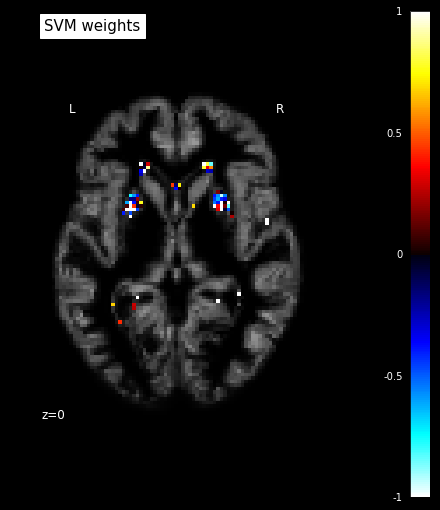
\includegraphics[scale=.3]{agepred.png}
\end{minipage}
\end{frame}

\note{

}

\begin{frame}
\frametitle{Feelings and emotions}
\begin{minipage}{.45\linewidth}
\begin{itemize}
\item Showing uncomfortable pictures while recording fMRI (BOLD).
\item Getting "bad feeling grades" back (1 to 5)
\item Train the model and evaluate it using K-Fold cross-validation
\end{itemize}
\end{minipage}
\hfill
\begin{minipage}{.45\linewidth}
\begin{center}
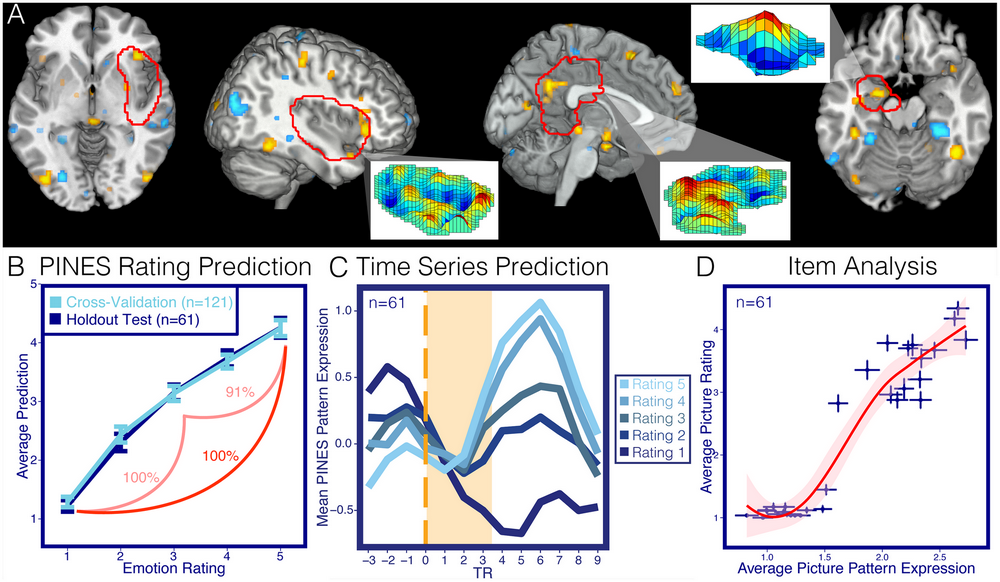
\includegraphics[scale=.2]{emotionpred.png}
\end{center}
\end{minipage}

\footnotetext[1]{
\tiny
Chang LJ, Gianaros PJ, Manuck SB, Krishnan A, Wager TD (2015) A Sensitive and Specific Neural Signature for Picture-Induced Negative Affect. PLoS Biol 13(6): e1002180. https://doi.org/10.1371/journal.pbio.1002180
}
\end{frame}

\note{

}

%%%%%%%%%%%%%%%%%%%%%%%%%
%%%%   CONCLUSION   %%%%%
%%%%%%%%%%%%%%%%%%%%%%%%%

\section{Conclusion}

\begin{frame}
\frametitle{Reverse inference Limits}
\begin{minipage}{.50\linewidth}
\begin{itemize}
\item Neuroimaging limits
\item Need for cognitive ontology 
(BrainMap Database)
\item Improving Reverse Inference
\end{itemize}
\end{minipage}
\hfill
\begin{minipage}{.45\linewidth}
\centering
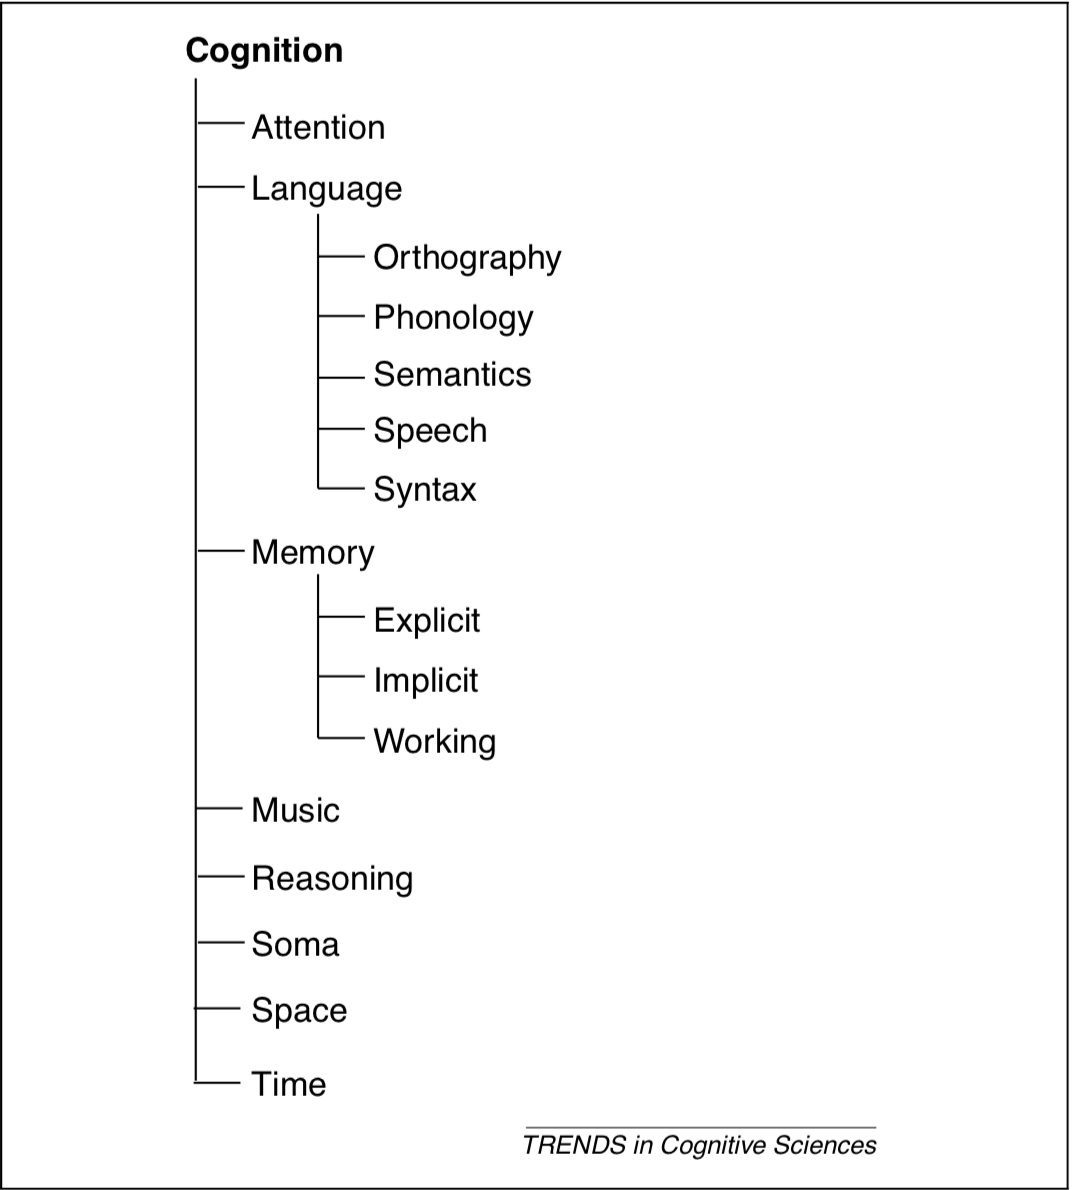
\includegraphics[scale=0.27]{BrainMapp.png}
\end{minipage}
\footnotetext[1]{
\tiny
Russell A. Poldrack, Can cognitive processes be inferred from neuroimaging data?, In Trends in Cognitive Sciences, Volume 10, Issue 2, 2006, Pages 59-63, ISSN 1364-6613, https://doi.org/10.1016/j.tics.2005.12.004.
}
\end{frame}

\begin{frame}
\frametitle{The future of machine learning for Neuroimaging}
\begin{itemize}
\item Be able to detect and understand physical disease such as ADHD
\item Be able to detect and understand mental disease such as schizophrenia
\item European Brain Project
\end{itemize}
\centering
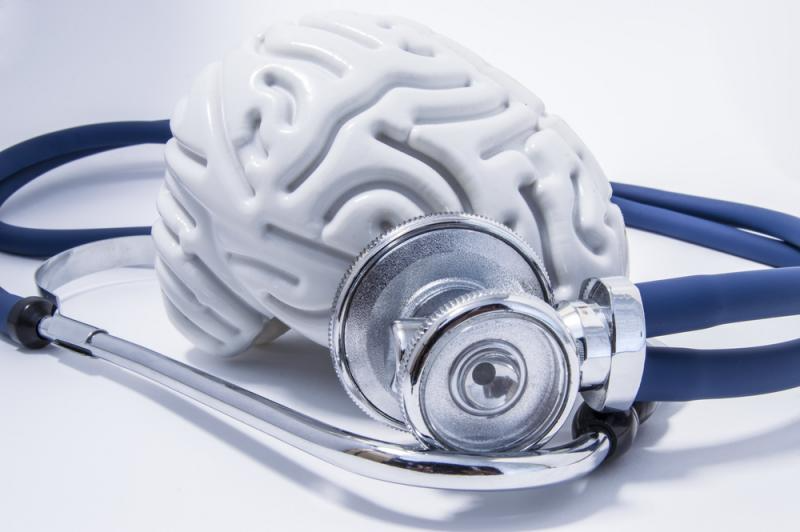
\includegraphics[scale=0.27]{future.png}
\end{frame}
%http://www.healthimaging.com/topics/molecular-imaging/neuroimaging/mri-technology-may-have-potential-diagnose-adhd-differentiate-subtypes

%https://www.rdmag.com/article/2017/07/utilizing-ai-machine-learning-better-understand-schizophrenia

\begin{frame}
\vfill
\centering
\begin{beamercolorbox}[sep=8pt,center,shadow=true,rounded=true]{title}
\usebeamerfont{title}
Questions ?
\end{beamercolorbox}
\vfill
\end{frame}



%%%%%%%%%%%%%%%%%%%%%%%%%%%%%%%%%%%%%%%%%%%%%%%%%%%%%%%%%%%%%%%%%%%%%%%%%%%%%%%%%%%%
% NE PAS MODIFIER CETTE PARTIE

%\begin{frame}[allowframebreaks, label=biblio]
%\printbibliography
%\end{frame}


\end{document}